
\documentclass[a4paper,12pt]{article}

\usepackage{ucs}
\usepackage[utf8x]{inputenc}
%\usepackage[latin1]{inputenc}
\usepackage[T1]{fontenc}

\usepackage[french]{babel}

\pagestyle{plain}

\usepackage{graphicx}
\usepackage{subfigure}
\DeclareGraphicsExtensions{.pdf,.eps,.jpg,.png,.gif}

\usepackage{color}
\definecolor{grey}{rgb}{0.9,0.9,0.9}
\definecolor{teal}{rgb}{0.0,0.5,0.5}
\definecolor{violet}{rgb}{0.5,0,0.5}

\usepackage{listings}
\usepackage{listingsutf8}
\lstloadlanguages{[Visual]C++}
\lstdefinestyle{listing}{
  language=Java,
  captionpos=t,
  inputencoding=utf8/latin1,
  extendedchars=true,
  resetmargins=true,
  xleftmargin=-60pt,
  xrightmargin=-70pt,
%  frame=single,
  numbers=left,
  numberstyle=\tiny,
  numbersep=5pt,
  breaklines=true,
  breakatwhitespace=true,
  showspaces=false,
  showstringspaces=false,
  showtabs=false,
  tabsize=2,
  basicstyle=\footnotesize\ttfamily,
  backgroundcolor=\color{grey},
  keywordstyle=\color{blue}\bfseries,
  commentstyle=\color{teal},
  identifierstyle=\color{black},
  stringstyle=\color{red},
  numberstyle=\color{violet},
}
\lstset{style=listing}

%%%%%%%%%%%%%%%%%%%%%%%%%%%%%%%%%%%%%%%%%%%%%%%%%%%%%%%%%%%%

\author{
  Quentin \textsc{Augrain}, Florent \textsc{Mallard} \\ \\
  INSA de Rennes \\
  5INFO
}

\title{Projet de Modélisation et Ingénierie du vivant}

\begin{document}
\maketitle

\section{Tutorial}

Question 1: As stated in the commentaries of the function, there are two phases in the main loop :
\begin{itemize}
    \item Move the world;
    \itme Display the world.
\end{itemize}

That means that the function will first compute the next move, and then display the new position. For now the computation does nothing, it is still to implement.

Question 2: Nothing happens. Even though we do compute the forces, we do not apply them to the mesh, which results in no changes on the screen.
\begin{figure}
  \centering
  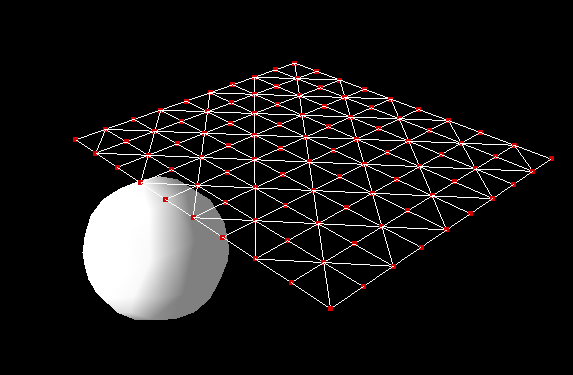
\includegraphics{q2.png}
  \caption{No changes are visible even if the forces are not the same.}
  \label{fig:q2}
\end{figure}

Question 3: Now that we apply the forces to the mesh, it falls ignoring the ball, and disappears.

Question 4 : In order to freeze the first row, we need to nullify the forces applied to those particles. We counted 10 particles, so we set a loop in the Simulator::Update() function, as shown in \textsc{Figure} \ref{fig:q4}.
\begin{figure}
  \centering
  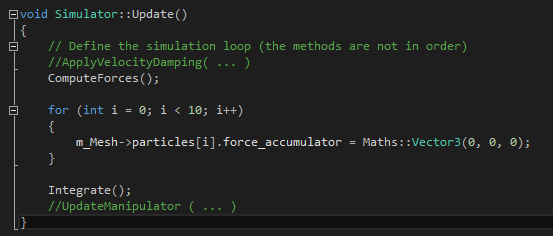
\includegraphics{q4.png}
  \caption{The first row remains fix.}
  \label{fig:q4}
\end{figure}

Question 5 : The behaviour is a bit strange, because the particles of the mesh move up and down until they disappear (except the first row).
\textsc{Figure} \ref{fig:q5} shows our implementation.
\begin{figure}
  \centering
  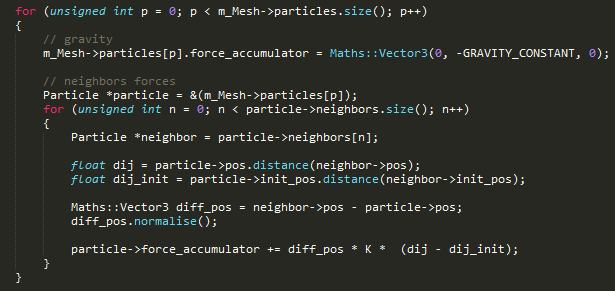
\includegraphics{q5.png}
  \caption{Update each neighbor for each particle.}
  \label{fig:q5}
\end{figure}

Question 6 : The dt parameter defines the speed of the simulation. The more little the the value, the slower the simulation goes. It is so because we compute the position of the particles and the forces applying to them after a very short amount of time, so it hasn't moved a lot.
K defines the stifness. It is a kind of elasticity which will help obtaining the "hanging curtain" effect desired.
But knowing that, we haven't been able to keep the simulation stable.

\lstinputlisting[caption=Un fichier C++...]{alea.cpp}

\end{document}
